\documentclass{beamer}

\usepackage{beamerthemeHannover,graphics,amsmath,bm}
\usepackage{Sweave}

\title[Ordinal Invariance]{Testing for Measurement Invariance with
  respect to an Ordinal Variable}
\author{Ed Merkle\inst{1} \and Jinyan Fan\inst{2} \and Achim Zeileis\inst{3}}
\institute{\inst{1} University of Missouri \and \inst{2} Auburn
  University \and \inst{3} Universit\"{a}t Innsbruck}
\date{\ }
%\date{Supported by NSF grant SES-1061334}

\begin{document}

\frame{\titlepage}

\section{Background}
% Define measurement invariance
\frame{
  \frametitle{Measurement Invariance}
  \begin{itemize}
    \item Measurement invariance: Sets of tests/items consistently
      assigning scores across diverse groups of individuals.\\ \ \\
    \item Commonly studied via factor analysis (today's focus) and
      item response models.\\ \ \\
    \item Focal problem: How do we test for measurement invariance
      with respect to an ordinal auxiliary variable, in a way that
      ``respects'' the fact that the variable is ordinal?
  \end{itemize}}

% FA path diagram, types of MI
\frame{
  \frametitle{Example (13--14 years)}
  \begin{center}
      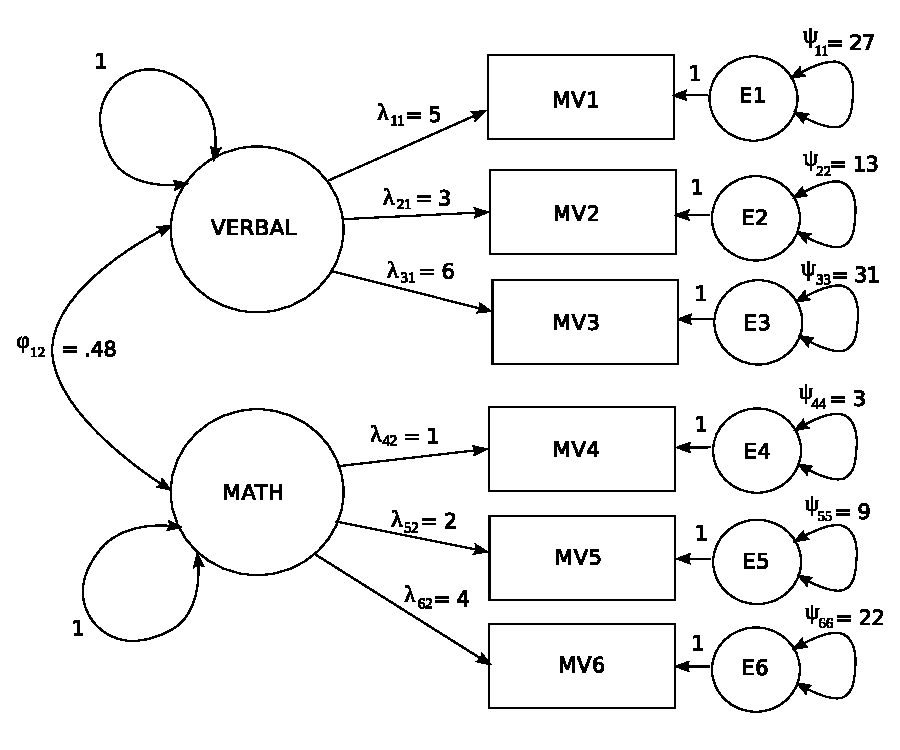
\includegraphics[height=3in]{../psychoco2012/model_under16.pdf}
  \end{center}}

\frame{
  \frametitle{Example (15--16 years)}
  \begin{center}
      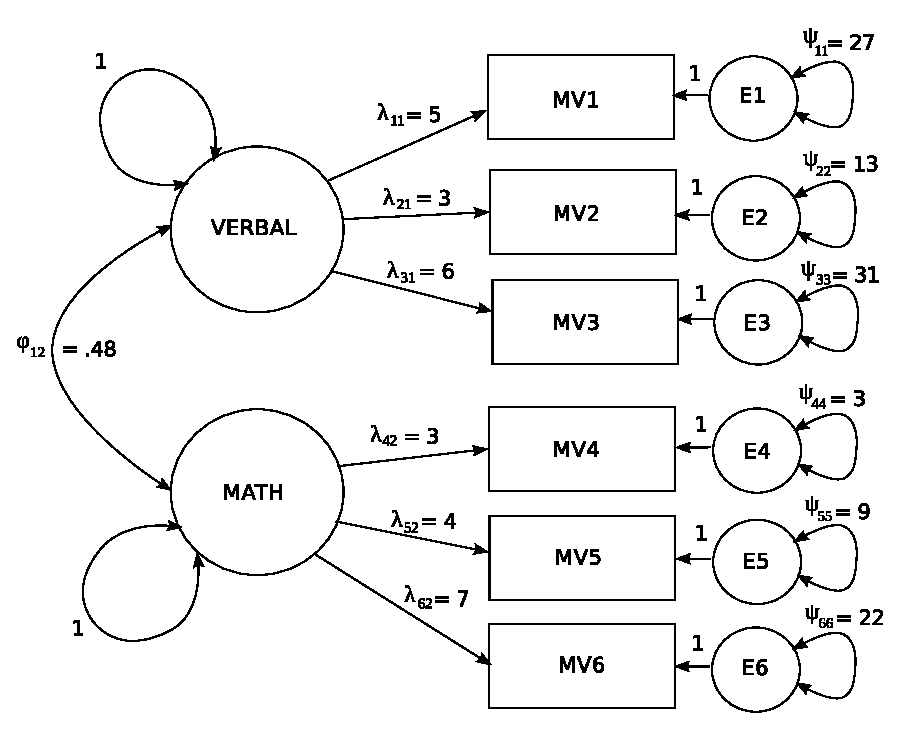
\includegraphics[height=3in]{../psychoco2012/model_over16.pdf}
  \end{center}}

\frame{
  \frametitle{Example (17 years)}
  \begin{center}
      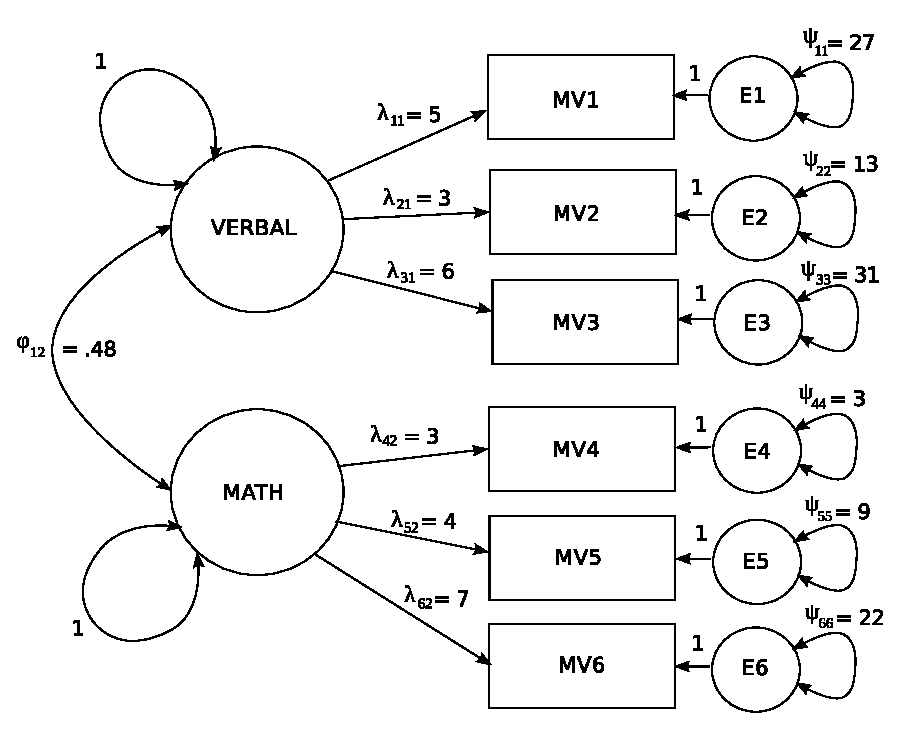
\includegraphics[height=3in]{../psychoco2012/model_over16.pdf}
  \end{center}}

\frame{
  \frametitle{Outline}
  \begin{itemize}
    \item The traditional way to test for measurement invariance here
      involves multiple-group models and likelihood ratio tests.
      However, these tests treat the ordinal variable as unordered.
      In this talk, we:
      \begin{itemize}
        \item Review last year's family of measurement invariance
          tests, which can be 
          used when the auxiliary variable is continuous.
        \item Present new test statistics to deal with situations when the
          auxiliary variable is ordinal.
        \item Illustrate the statistics and compare them to
          traditional methods.
      \end{itemize}
  \end{itemize}}

\section{Theory}
% Define as theta_i = theta_0, i=1,..,n
\frame{
  \frametitle{Hypotheses}
  \begin{itemize}
    % \item There exist many types of measurement invariance,
    %   based on specific subsets of parameters being allowed
    %   to vary across individuals (e.g., Meredith, 1993).\\ \ \\
    \item Hypothesis of ``full'' measurement invariance:\\
      \begin{center}
          $H_0: \bm{\theta}_i = \bm{\theta}_0, i=1,\ldots,n$\\
          $H_1: \text{Not all the }\bm{\theta}_i = \bm{\theta}_0$
      \end{center}
      where $\bm{\theta}_i = (\lambda_{i, 1, 1}, \dots, \psi_{i, 1, 1}, \dots, \varphi_{i, 1, 2})^\top$
      is the full $p$-dimensional parameter vector for individual $i$.
  \end{itemize}}

% Too difficult to assess, so use an auxiliary variable to place
% people in meaningful groups
  % continuous vs categorical auxiliary variable
\frame{
  \frametitle{Hypotheses}
  \begin{itemize}
    \item $H_0$ from the previous slide is difficult to fully assess
      due to all the ways by which individuals may differ.\\ \ \\
    \item If our auxiliary variable of interest is continuous (i.e.,
      we do not know the groups in advance), we could conduct 
      a LR or LM test for each possible pair of groups, then take the maximum.
      Requires different critical values!
  \end{itemize}}

\frame{
  \frametitle{Lack of Grouping}
  \begin{center}
      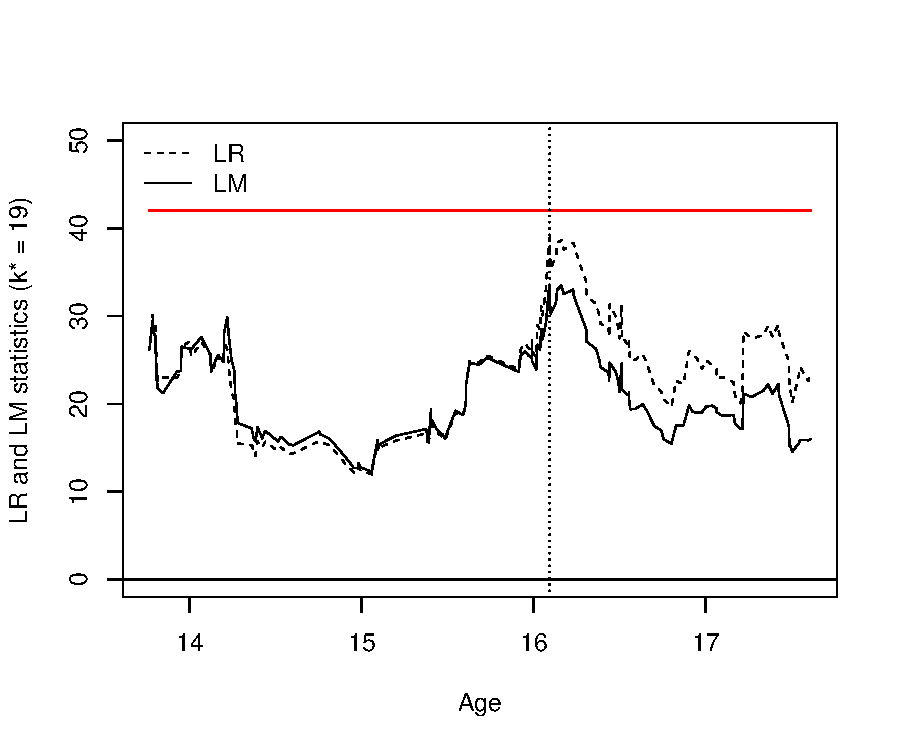
\includegraphics[height=3in]{../psychoco2012/paper-lm-lr-19.pdf}
  \end{center}
}

\frame{
  \frametitle{Instability Tests}
  \begin{itemize}
    \item The tests presented last year expand on this idea, removing
      the need to fit more than one model.\\ \ \\
    \item Idea: Fit a ``reduced'' model to the data (assuming, e.g.,
      that parameters are equal across groups).  Examine how
      individuals' {\em scores} vary across the continuous auxiliary
      variable.
  \end{itemize}}

\frame{
  \frametitle{Scores}
  \begin{itemize}
    \item What are scores?
   \begin{itemize}
    \item The traditional way to obtain maximum likelihood estimates
      involves choosing estimates $\widehat{\bm{\theta}}$ so that\\
  \begin{center}
  $\frac{\partial}{\partial \bm{\theta}} \displaystyle\sum_{i=1}^{n} \log
\text{L}({\bm{x}}_i, {\bm{\theta}}) \big |_{\bm{\theta} = \widehat{\bm{\theta}}} = 
  {\bm 0}$
  \end{center}\ \\ \ \\
    \item Individual terms of this summation are the scores\\
  \begin{center}
  $s(\hat{{\bm \theta}}; \bm{x}_i) = \frac{\partial}{\partial \bm{\theta}} \log
\text{L}({\bm{x}}_i, {\bm{\theta}}) \big |_{\bm{\theta} =
  \widehat{\bm{\theta}}}$
  \end{center}\ \\ \ \\
    \item $s(\hat{{\bm \theta}}; \bm{x}_i)$ can be conceptualized 
      as a residual for individual $i$: close to ${\bm 0}$ is good,
      far from ${\bm 0}$ is not so good. 
  \end{itemize}
 \end{itemize}}

\frame{
  \frametitle{Instability Tests}
  \begin{itemize}
    \item Under measurement invariance, parameter estimates should
      roughly describe everyone equally well.  So, people's scores
      should fluctuate around zero as we move up the auxiliary variable.\\ \ \\
    \item If measurement invariance is violated, the scores should
      stray from zero around specific points of the auxiliary variable.
  \end{itemize}}

\begin{frame}[fragile]
  \frametitle{Aggregating Scores}
 % define cumulative scores and other notation
  \begin{itemize}
    \item We need a way to aggregate scores across individuals so that we
      can draw some general conclusions.  We define a {\em cumulative score
      process}, which is advantageous because we know its distribution
      under $H_0$:
      \begin{itemize}
        \item Order individuals by the auxiliary variable.\\ \ \\
        \item Define $t \in (0, 1)$.
          The empirical cumulative score process is defined by:\\
  \begin{equation*}
    \bm{B}(t; \hat{\bm{\theta}}) = 
      {\bm{\widehat I}}^{-1/2} \frac{1}{\sqrt{n}}
    \displaystyle\sum_{i=1}^{\lfloor nt 
      \rfloor} s(\hat{\bm{\theta}} ; \bm{x}_i).
    \end{equation*}
  where $\lfloor nt \rfloor$ is the integer part of $nt$
  and $\bm{\widehat I}$ is some consistent covariance matrix estimate, e.g.,
  the observed information matrix ${\bm{I}}(\widehat{{\bm{\theta}}})$.
      \end{itemize}
  \end{itemize}
\end{frame}


\begin{frame}[fragile]
  \frametitle{Tests}
 % show that cumulative scores follow a Brownian bridge under H_0
  \begin{itemize}
    \item Under the hypothesis of
      measurement invariance, a functional central limit
      theorem holds:
  \begin{equation*}
  {\bm{B}}(\cdot; \widehat{{\bm{\theta}}}) \overset{d}{\rightarrow} {\bm B}^{0}(\cdot),
  \end{equation*}
 where ${\bm B}^{0}(\cdot)$ is a $p$-dimensional Brownian bridge.\\ \ \\

   \item Testing procedure: Compute an aggregated statistic of the empirical
     score process and compare with corresponding quantile of aggregated
     Brownian motion.\\ \ \\

    \item Test statistics: Special cases include double maximum (DM),
      Cram\'er-von Mises (CvM), maximum of LM statistics.
  \end{itemize}
\end{frame}


\begin{frame}[fragile]
  \frametitle{Tests}

\begin{itemize}
  \item Test statistics aggregate over parameters (columns) $j = 1,
    \dots, k$ and observations (rows) $i = 1, \dots, n$,
    employing different norms.
  \item Special cases:
    \begin{eqnarray*}
      \mathit{DM}      & = & \max_{i = 1,\dots, n} \max_{j = 1, \dots, k} | {\bm B}(\hat {\bm \theta})_{ij} |,\\
      \mathit{CvM}     & = & n^{-1} \sum_{i = 1,\dots, n} \sum_{j = 1, \dots, k} {\bm B}(\hat {\bm \theta})_{ij}^2, \\
      \max \mathit{LM} & = & \max_{i = \underline{i}, \dots, \overline{\imath}} ~
                             \left\{ \frac{i}{n} \left( 1 - \frac{i}{n} \right) \right\}^{-1}
                             \sum_{j = 1, \dots, k} {\bm B}(\hat {\bm \theta})_{ij}^2.
    \end{eqnarray*}
  \item ${\bm B}(\hat {\bm \theta})_{ij}$ is short for $\bm{B}(i/n; \hat{\bm{\theta}})_j$.
\end{itemize}
\end{frame}

\frame{
  \frametitle{Illustration}
  \begin{center}
      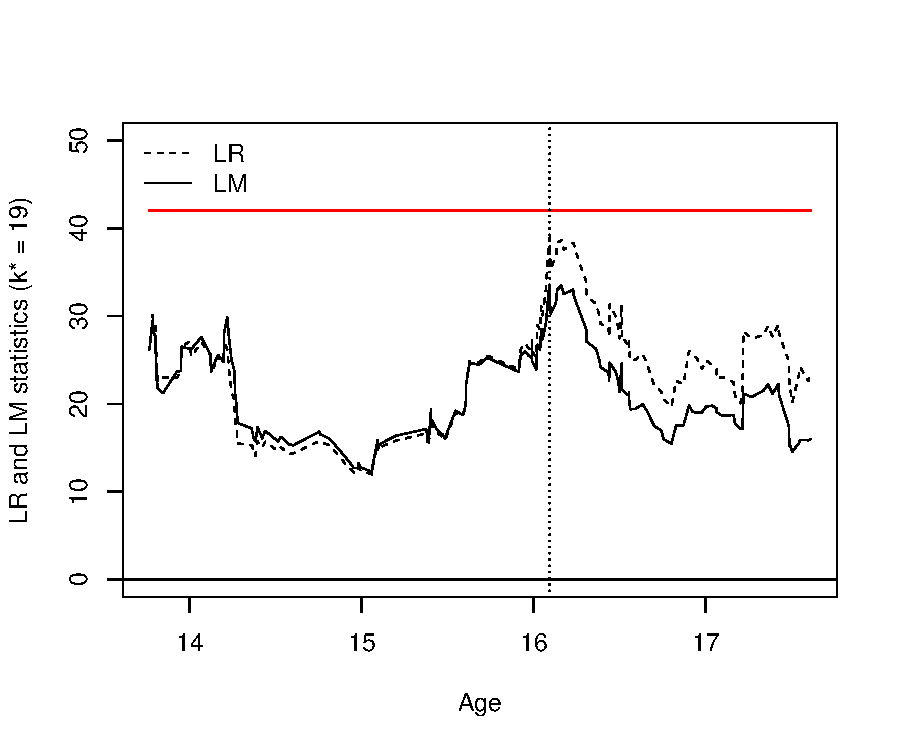
\includegraphics[height=3in]{../psychoco2012/paper-lm-lr-19.pdf}
  \end{center}
}

\section{Ordinal Tests}
\frame{
  \frametitle{Ordinal vs Continuous Tests}
  \begin{itemize}
    \item Last year, we showed that the above tests have adequate
      power to be useful in practice.\\ \ \\
    \item However, the tests require a unique ordering of individuals
      w.r.t.\ the auxiliary variable.\\ \ \\
    \item If the auxiliary variable is ordinal, we have a large number
      of ties.  What to do?
  \end{itemize}}

\frame{
  \frametitle{Tests along Ordinal Variables}
  \begin{itemize}
    \item To obtain a test statistic in the ordinal case, we allow all
      individuals with the same value of the 
      auxiliary variable to simultaneously enter into the cumulative
      sum.  We then apply the same functionals that were used in the
      continuous case.
    \item Critical values are obtained by summing bins of a Brownian
      bridge, where bin sizes match the observed bin sizes of the 
      ordinal variable.  This allows us to treat ordinal auxiliary
      variables as truly ordinal, which no existing methods (to our
      knowledge) can do.
  \end{itemize}}

\frame{
  \frametitle{Tests along Ordinal Variables}
  \begin{itemize}
    \item Instead of aggregating over all $i = 1, \dots, n$, aggregate
      only over $i_\ell = \lfloor n \cdot t_\ell\rfloor$ for the cumulative proportions
      $t_\ell$ ($\ell = 1, \dots, m$).
    \item Tests: Obtain ordinal versions of the max LM test and (weighted) double maximum test.
      % Additionally use LM-type test that does not exploit ordering.
    \begin{eqnarray*}
      \mathit{WDM}_o & = & \max_{i \in \{i_1, \dots, i_m \}} ~ \left\{ \frac{i}{n} \left( 1 - \frac{i}{n} \right) \right\}^{-1}      
                             \max_{j = 1, \dots, k} | {\bm B}(\hat {\bm \theta})_{ij} |,\\
      \max \mathit{LM}_o & = & \max_{i \in \{i_1, \dots, i_m \}} ~
                             \left\{ \frac{i}{n} \left( 1 - \frac{i}{n} \right) \right\}^{-1}
                             \sum_{j = 1, \dots, k} {\bm B}(\hat {\bm \theta})_{ij}^2.\\
%      \mathit{LM}_\mathit{uo} & = & \sum_{\ell = 1, \dots, m+1} \sum_{j = 1, \dots, k}
%        \left( {\bm B}(\hat {\bm \theta})_{i_\ell j} - {\bm B}(\hat {\bm \theta})_{i_{\ell - 1}j} \right)^2.
    \end{eqnarray*}
  \end{itemize}}

\subsection{Simulations}

\frame{
  \frametitle{Simulation 1}
  \begin{itemize}
    \item Simulation 1:
      \begin{itemize}
        \item Two-factor model, with each factor having three unique
          indicators.
        \item Measurement invariance violation in three unique
          variance parameters, growing as we move up the ordinal
          variable.
        \item Sample size in $\{120, 480, 960\}$.
        \item Levels of the ordinal variable in $\{4, 8, 12\}$.
        \item Four test statistics (two new statistics, the
          multiple group LRT, and the unordered Lagrange multiplier test).
      \end{itemize}
  \end{itemize}}

\frame{
  \frametitle{Simulation 1}
  % Graph of results
  \begin{center}
      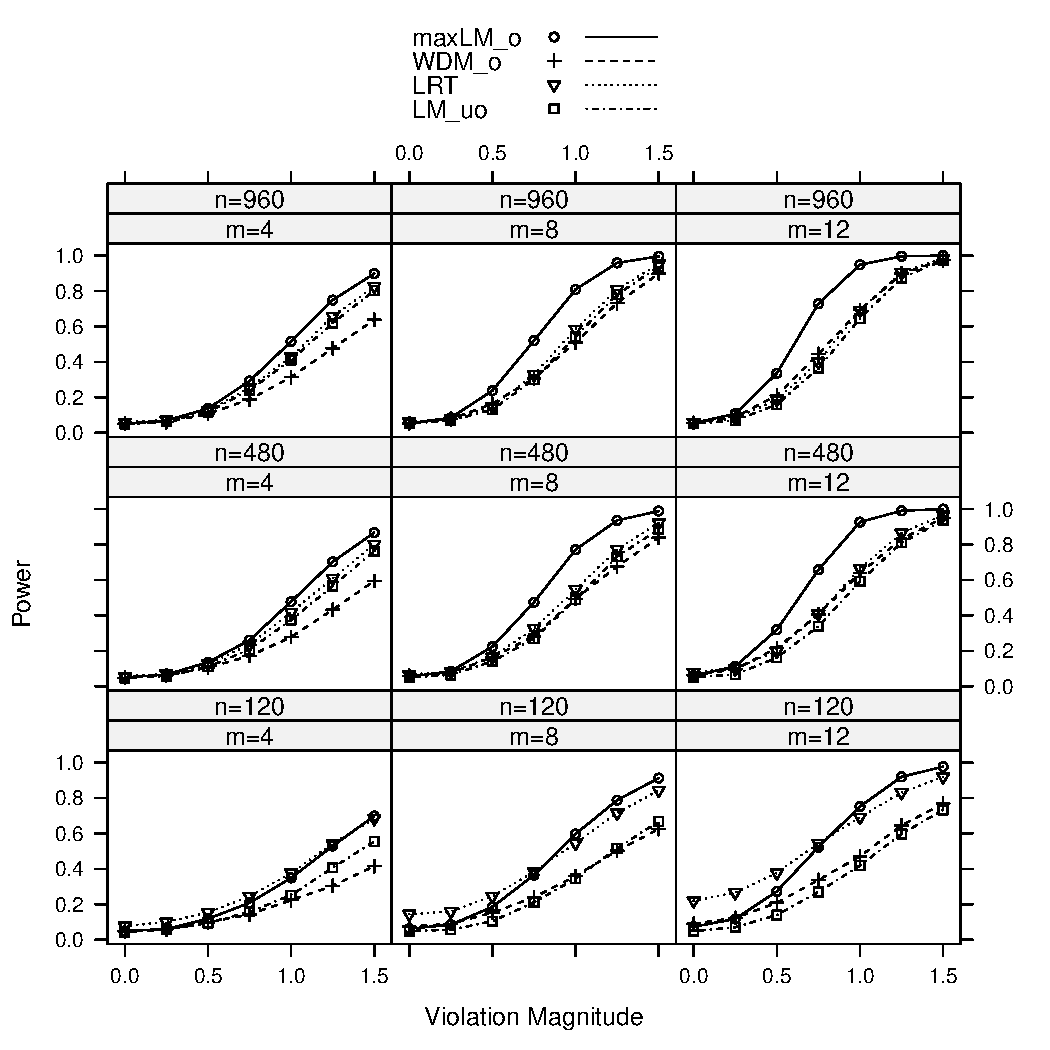
\includegraphics[height=3in]{ordinal-sim1res}
  \end{center}
}

\frame{
  \frametitle{Simulation 2}
  \begin{itemize}
    \item Simulation 2: Are the proposed test statistics less
      sensitive to large $n$, as compared to the analogous likelihood
      ratio test (e.g., Bentler and Bonnett, 1980)?
      \begin{itemize}
        \item Same two-factor model from before.
        \item Small measurement invariance violation (0, 0.5, \dots,
          3 standard errors apart) in all unique
          variance parameters at a middle level of the ordinal auxiliary
          variable.
        \item Sample size in $\{1200, 4800, 9600\}$.
        \item Levels of the ordinal variable in $\{4, 8, 12\}$.
        \item Four test statistics (two new statistics, the
          multiple group LRT, and the unordered Lagrange multiplier test).
      \end{itemize}
  \end{itemize}}

\frame{
  \frametitle{Simulation 2}
  % Graph of results
  \begin{center}
      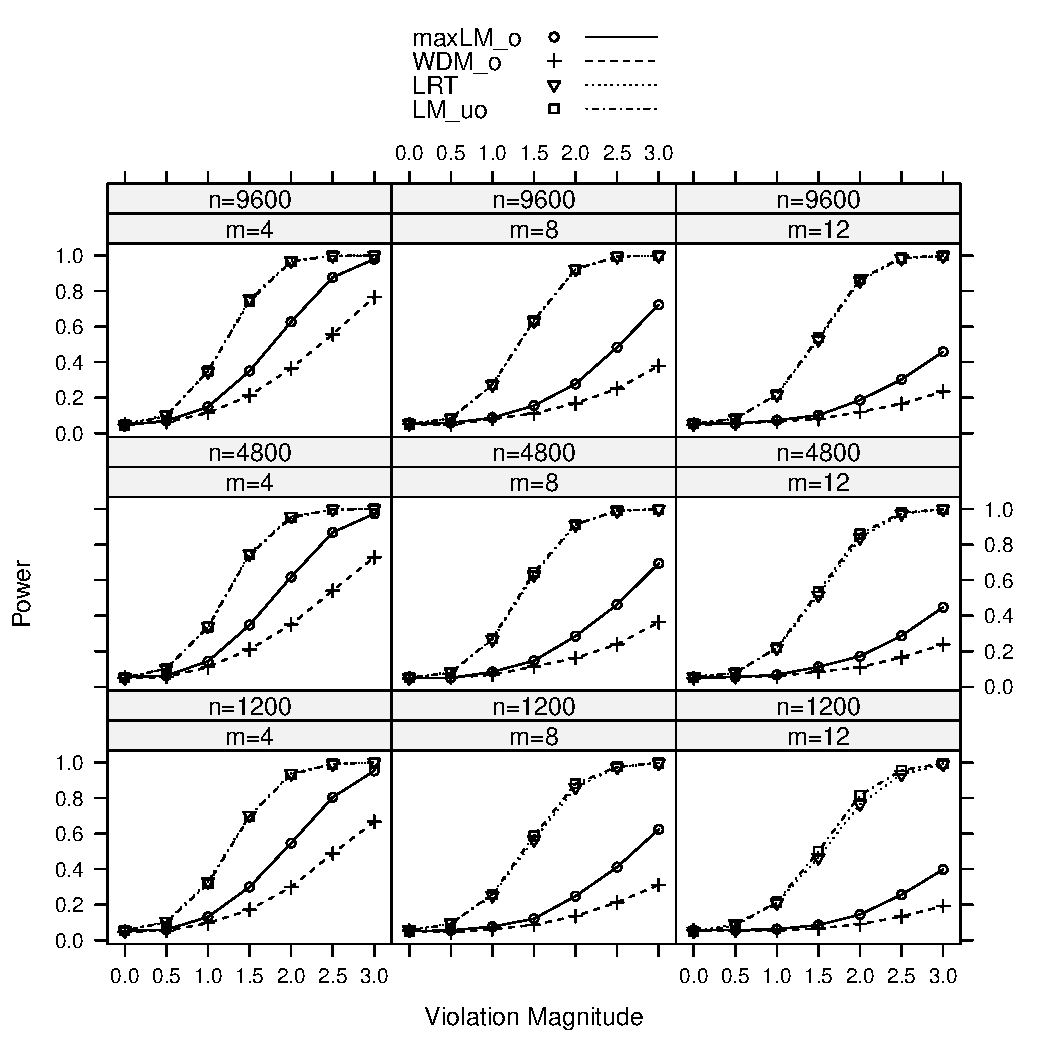
\includegraphics[height=3in]{ordinal-sim2res}
  \end{center}
}

\frame{
  \frametitle{Simulations}
  \begin{itemize}
  \item Conclusions from ordinal simulations
    \begin{itemize}
    \item In the ordinal scenarios examined, the ordered Lagrange multiplier
      statistic has higher power to detect measurement invariance
      violations than does the traditional LRT.
    \item The ordered Lagrange multiplier statistic is also less
      sensitive to minor invariance violations at large $n$, as
      compared to the traditional LRT (the ordered double-max
      statistic is also less sensitive, but its power is generally
      poor).
    \item The ordered Lagrange multiplier statistic has good potential
      for practical application (though a downside is that critical
      values must be simulated).
    \end{itemize}
  \end{itemize}}

\subsection{Example}

\frame{
  \frametitle{Example}
  \begin{itemize}
    \item Example: A small number of scales have been developed to
      measure gratitude in adults.  Can these scales also be used with
      youth? (Froh, Fan, et al., 2011)
      \begin{enumerate}
        \item $n=1,401$ youth ages 10--19 complete three gratitude
          scales.  Age groups are \{10--11, 12--13, 14, 15, 16,
          17--19\}.
        \item Measurement invariance examined via factor analyses of
          each individual scale (one-factor models), with
          increasingly-restricted parameters.
      \end{enumerate}
  \end{itemize}}

\frame{
  \frametitle{Example}
  \begin{itemize}
    \item The large sample size made the authors suspicious about
      significant likelihood ratio tests of model fit, making it difficult
      to draw final conclusions about measurement invariance.
      \begin{itemize}
        \item GQ6 scale: Compare congeneric model to tau-equivalent model,
          obtain $\chi^2_{20}=38.08, p=.009$
        \item GAC scale: Compare tau-equivalent model to parallel model,
          obtain $\chi^2_{20}=167.72, p<.001$\\ \ \\
      \end{itemize}
    \item To use our proposed statistics in each case, we fit the
      restricted model and test the parameters that are freed in the
      less-restricted model.
  \end{itemize}}

\begin{frame}[fragile]
  \frametitle{GQ6 Results}
  \begin{itemize}
    \item LRT implies the congeneric model is better, whereas our
      proposed statistics imply the tau-equivalent model is as good
      ($WDM_{o}=2.91, p=.06$; $\max LM_o = 11.16, p=.10$)
  \end{itemize}
  \begin{center}
      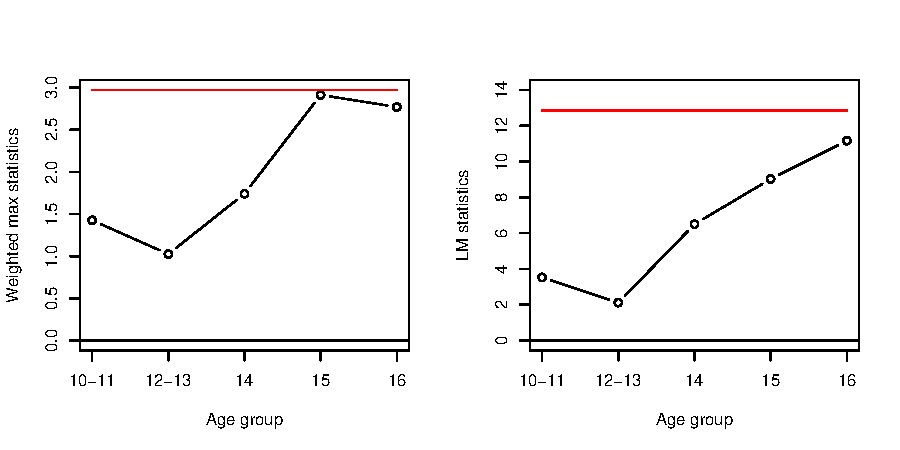
\includegraphics[height=2in]{ordinal-gq6res.pdf}
  \end{center}
\end{frame}

\begin{frame}[fragile]
  \frametitle{GAC Results}
  \begin{itemize}
    \item LRT implies the tau-equivalent model is better, and our
      proposed statistics agree ($WDM_{o}=6.55, p<.01$; $\max LM_o =
      113.13, p<.01$)
  \end{itemize}
  \begin{center}
      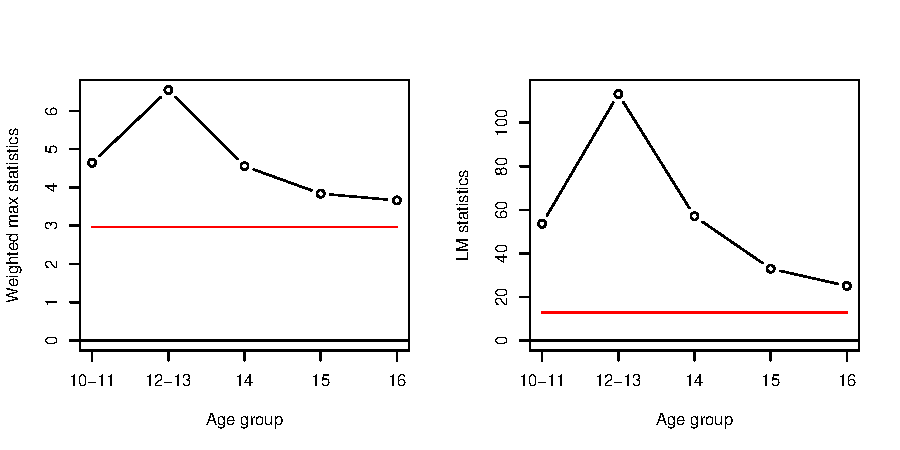
\includegraphics[height=2in]{ordinal-gacres.pdf}
  \end{center}
\end{frame}

\section{Conclusions}
\frame{
  \frametitle{General Conclusions}
  \begin{itemize}
    \item The family of measurement invariance tests considered here 
      usefully extends to the ordinal case:
      \begin{itemize}
        \item Increased sensitivity to ``ordinal'' violations.
        \item Decreased sensitivity to anomalous violations induced by
          large $n$.
        \item Ability to test at low $n$, where
          multiple-group models are not feasible (the proposed tests
          only require the ``reduced'' model).
      \end{itemize}
  \end{itemize}}

\begin{frame}[fragile]
  \frametitle{Software}
  \begin{itemize}
    \item R currently has functionality to carry out the proposed
      tests for general SEMs:
      \begin{itemize}
        \item \texttt{lavaan} for model estimation, with score
          extraction included in recent versions via \verb+estfun()+.\\ \ \\
        \item \texttt{strucchange} for carrying out the proposed
          tests.\\ \ \\
        \item See \url{http://semtools.r-forge.r-project.org/} for
          papers and relevant code.
      \end{itemize}
  \end{itemize}
\end{frame}

\begin{frame}[fragile]
  \frametitle{Acknowledgements}
  \begin{itemize}
    \item Support from NSF grant SES-1061334\\ \ \\
    \item Yves Rosseel, \verb+lavaan+ development\\ \ \\
  \end{itemize}
\end{frame}

\frame{
  \frametitle{}
  \begin{itemize}
  \item Questions?
  \end{itemize}}

\end{document}
